\chapter{はじめに}
\label{ch:intro}

\quad

本章では,本研究を始めるにあたっての動機,および本論文の構成を示す。

\section{研究背景}
\label{sec:research_bg}

日本企業のRPA(Robotics Process Automation~\cite{yasuhiro2017rpa})導入率は全体で38\%、中堅 ・ 中小企業では25\%となっており、非常に少ないことがわかる。(図~\ref{fig:rpa_rate})
また、大企業と中堅 ・ 中小企業の間に20\%以上の差があり、技術や規模による格差も見て取れる。
これらの原因となっており要因として考えられることは、大きく分けて2つある。1つ目は、RPAには専門領域と非専門領域が存在するということである。
専門領域はPC上の操作や、デジタルの領域における処理である。いっぽうで、紙媒体の処理等の、アナログの世界で行われる処理は非専門領域としている。特に、手書きの文字や画像の認識を高い精度を保ちながら自z動で行うことは、現代では非常に困難なことである。縦書き文字横書き文字が混在していたり、旧字体や特殊文字等の組み合わせも考えられるため。例外的な処理までを自動で行う必要があるからである~\cite{d-analyzer2019rpa}。2つ目の原因は、紙媒体の業務を行っているコミュニティのIT知識の乏しさにある。詳しくは次のセクションで説明する。このような現状を踏まえて、次章からは、OCR技術を使用したアプローチを提案する。

\clearpage
\begin{figure}[htbp]
\centering
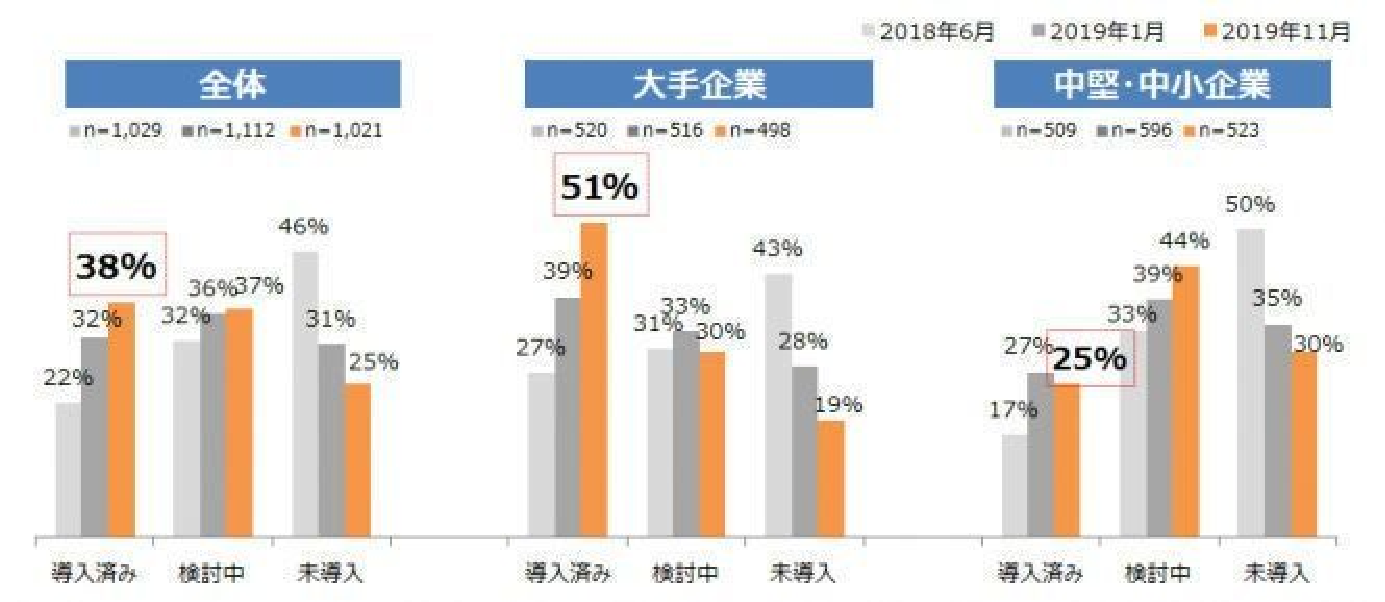
\includegraphics[scale = 0.6]{img/rpa_rate.pdf}
\caption{企業のRPA導入率}
\label{fig:rpa_rate}
\end{figure}%

\section{研究目的}
\label{sec:research_purpose}

本研究の目的は、IT知識が乏しく、紙媒体の業務を行っているコミュニティを中心に。RPAを使用して紙媒体の処理を自動で行うシステムを作成することである。
具体的な内容に入る前に、紙媒体の業務とIT知識の関連性について深堀りする。
日本で働く人事 ・ 総務担当者に、「紙媒体中心の業務で不便を感じたことがあるか?」とアンケートを取ったところ、61\%が不便を感じたことがあると回答した。(図~\ref{fig:paper_media_survey})。上記の理由として、システム障害への恐怖感や、IT知識の乏しさが挙げられます。しかし、一連の流れをRPAにすることで、IT知識の有無に関わらず、システムを運用することを目指す。

\section{構成}
\label{sec_str}

本論文は6章構成になっている。第\ref{ch:intro}章では、本研究の背景や目的を述べる。第\ref{ch:rw}章では既存手法との比較や課題を述べる。本研究での実装手法を第\ref{ch:app}章で提案し、第\ref{ch:exp}章で実験と評価、第\ref{ch:eval}章で結果の考察を述べ、第\ref{ch:con}章でに本研究の総括を行う。

\begin{figure}[htbp]
\vspace{1cm}
\centering
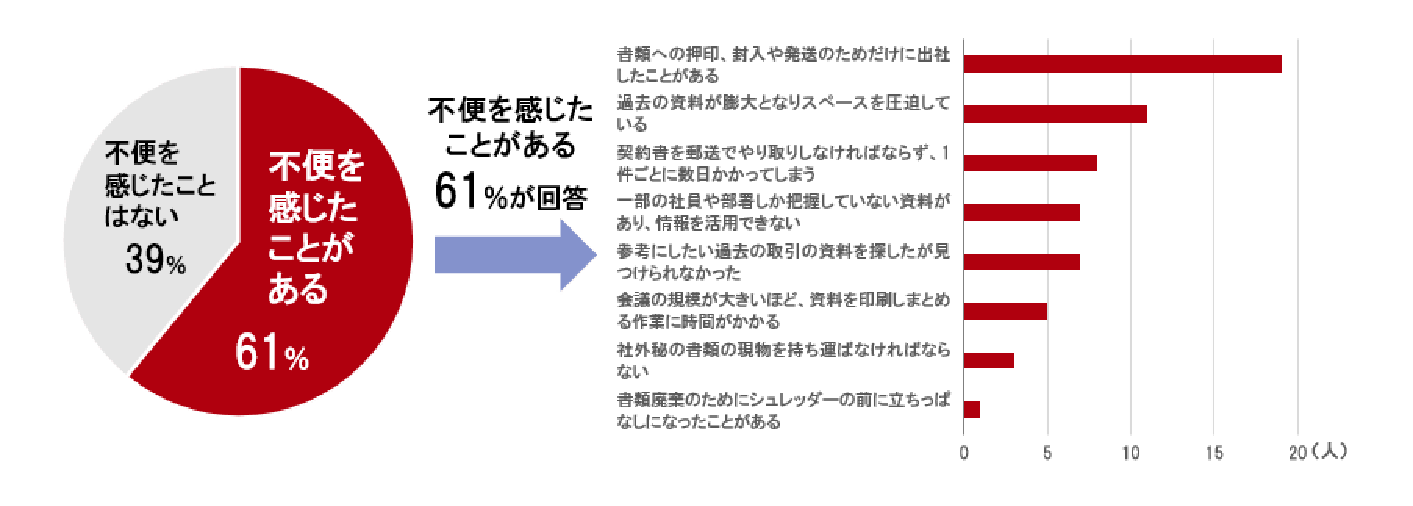
\includegraphics[scale = 0.6]{img/paper_media_survey.pdf}
\caption{紙媒体中心業務に関するアンケート}
\label{fig:paper_media_survey}
\end{figure}%
